% ------------------------------------------------------------------------------
% TYPO3 CMS 7.0 - What's New - Chapter "Backend User Interface" (Russian Version)
%
% @author	Michael Schams <schams.net>
% @license	Creative Commons BY-NC-SA 3.0
% @link		http://typo3.org/download/release-notes/whats-new/
% @language	Russian
% ------------------------------------------------------------------------------
% LTXE-CHAPTER-UID:		0fb2f94c-1065781a-e81383bc-81fae21b
% LTXE-CHAPTER-NAME:	Backend User Interface
% ------------------------------------------------------------------------------

\section{BackendUI}
\begin{frame}[fragile]
	\frametitle{Backend / Внутренний интерфейс}

	\begin{center}\huge{Глава 1:}\end{center}
	\begin{center}\huge{\color{typo3darkgrey}\textbf{Backend / Внутренний интерфейс}}\end{center}

\end{frame}

% ------------------------------------------------------------------------------
% LTXE-SLIDE-START
% LTXE-SLIDE-UID:		9ad538a8-da8ea8b9-91dad242-cd31f43e
% LTXE-SLIDE-ORIGIN:	fcbdd27c-e9005dff-0f4dd846-000ea412 English
% LTXE-SLIDE-TITLE:		In General
% LTXE-SLIDE-REFERENCE:	https://forge.typo3.org/issues/62333
% LTXE-SLIDE-REFERENCE:	https://forge.typo3.org/issues/62995
% LTXE-SLIDE-REFERENCE:	https://forge.typo3.org/issues/62158
% LTXE-SLIDE-REFERENCE:	https://forge.typo3.org/issues/61454
% ------------------------------------------------------------------------------

\begin{frame}[fragile]
	\frametitle{Backend / Внутренний интерфейс}
	\framesubtitle{Вкратце}

	\begin{itemize}
		\item Значительные изменения внешнего вида внутреннего интерфейса
		\item На базе Twitter Bootstrap версии 3.2.x
		\item Перерисованы все значки в стиле "tile"
		\item Значки используют шрифт Awesome версии 4.2.x
		\item Соответствующие изменения в основном меню слева
		\item Значки основного меню в стиле flat, цветной фон, монохромные/инверсные пиктограмы на фоне, скруглённые углы
		\item Ширину меню можно уменьшить, чтобы были видны лишь значки

	\end{itemize}

\end{frame}

% ------------------------------------------------------------------------------
% LTXE-SLIDE-START
% LTXE-SLIDE-UID:		18ff13c5-77e72827-34abc9a4-f3617864
% LTXE-SLIDE-ORIGIN:	0ae980b6-0d2ae6c6-52182f58-aaef69e3 English
% LTXE-SLIDE-TITLE:		Look & Feel (1)
% ------------------------------------------------------------------------------

\begin{frame}[fragile]
	\frametitle{Backend / Внутренний интерфейс}
	\framesubtitle{Вид и ощущение}

	\begin{figure}
		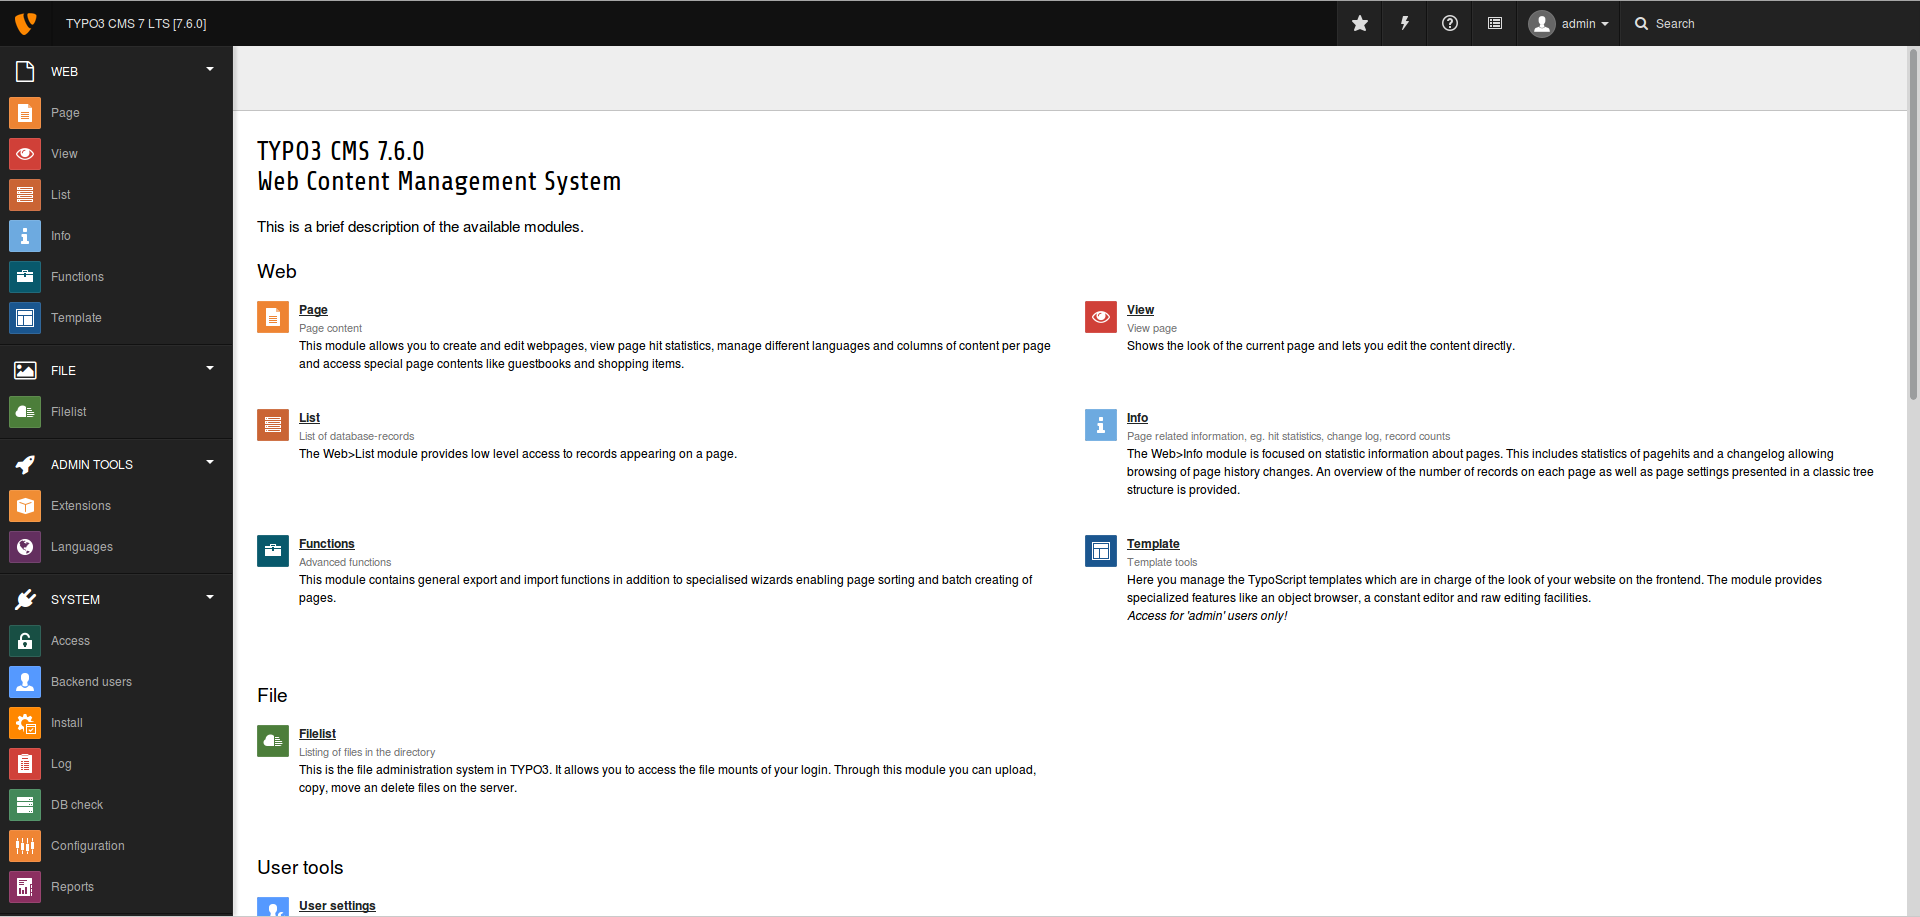
\includegraphics[width=0.90\linewidth]{BackendUserInterface/be-totalscreenshot1.png}
	\end{figure}

\end{frame}

% ------------------------------------------------------------------------------
% LTXE-SLIDE-START
% LTXE-SLIDE-UID:		76b32c2e-7d1105af-94a85776-17238f6e
% LTXE-SLIDE-ORIGIN:	250b123b-2c0bfce4-506f16b0-629baa10 English
% LTXE-SLIDE-TITLE:		Look & Feel (2)
% ------------------------------------------------------------------------------

\begin{frame}[fragile]
	\frametitle{Backend / Внутренний интерфейс}
	\framesubtitle{Вид и ощущение}

	\begin{figure}
		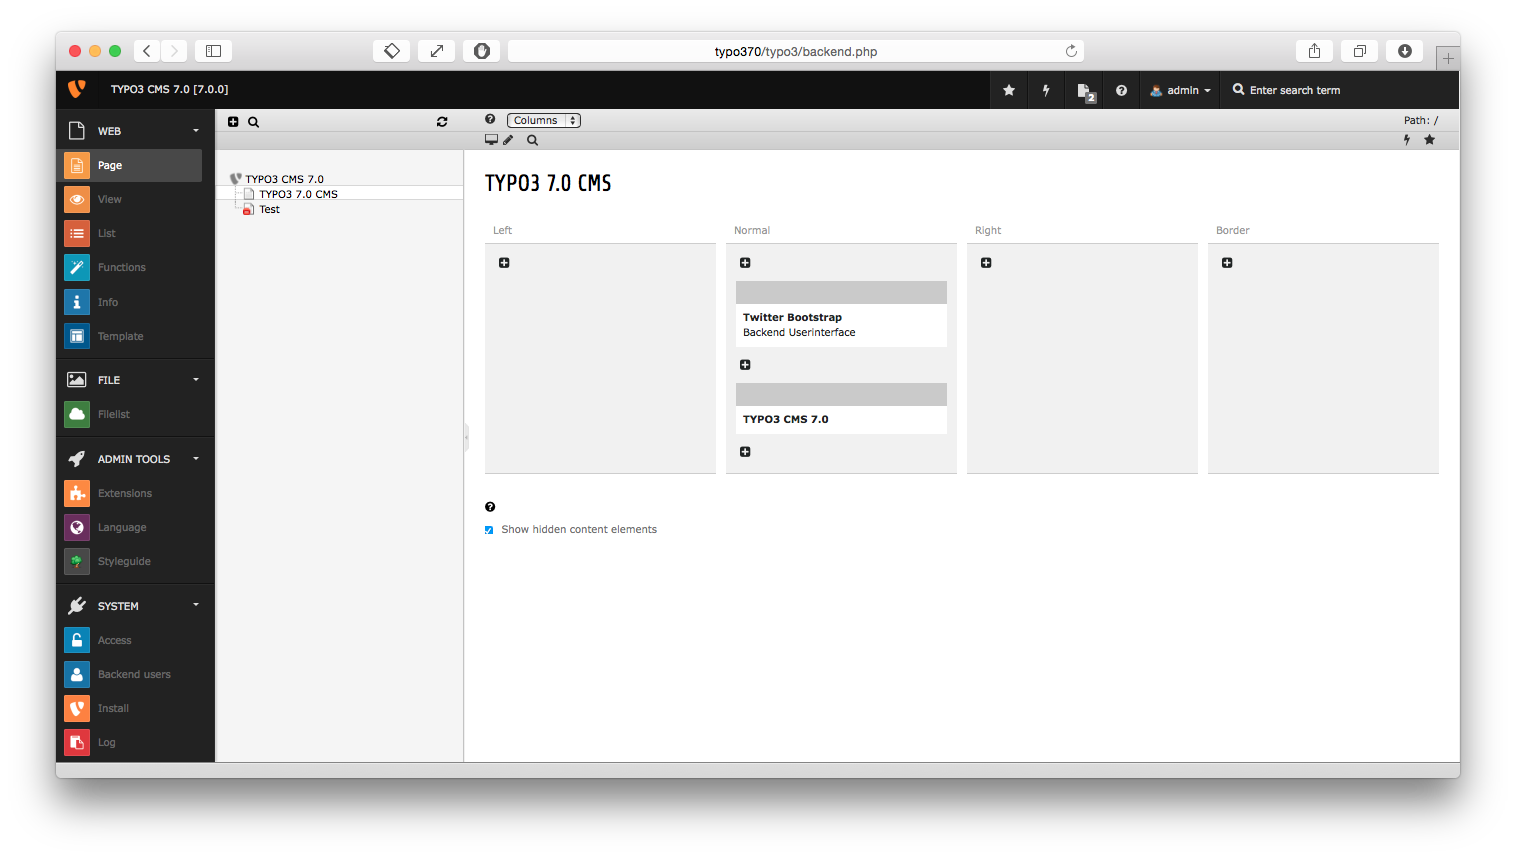
\includegraphics[width=0.90\linewidth]{BackendUserInterface/be-totalscreenshot2.png}
	\end{figure}

\end{frame}

% ------------------------------------------------------------------------------
% LTXE-SLIDE-START
% LTXE-SLIDE-UID:		2f490577-a46f9807-f8c52f1b-4c14eaab
% LTXE-SLIDE-ORIGIN:	2d4d33ee-071ae6ed-9f4d0c04-49361364 English
% LTXE-SLIDE-TITLE:		Look & Feel (3)
% ------------------------------------------------------------------------------

\begin{frame}[fragile]
	\frametitle{Backend / Внутренний интерфейс}
	\framesubtitle{Вид и ощущение}

	\begin{figure}
		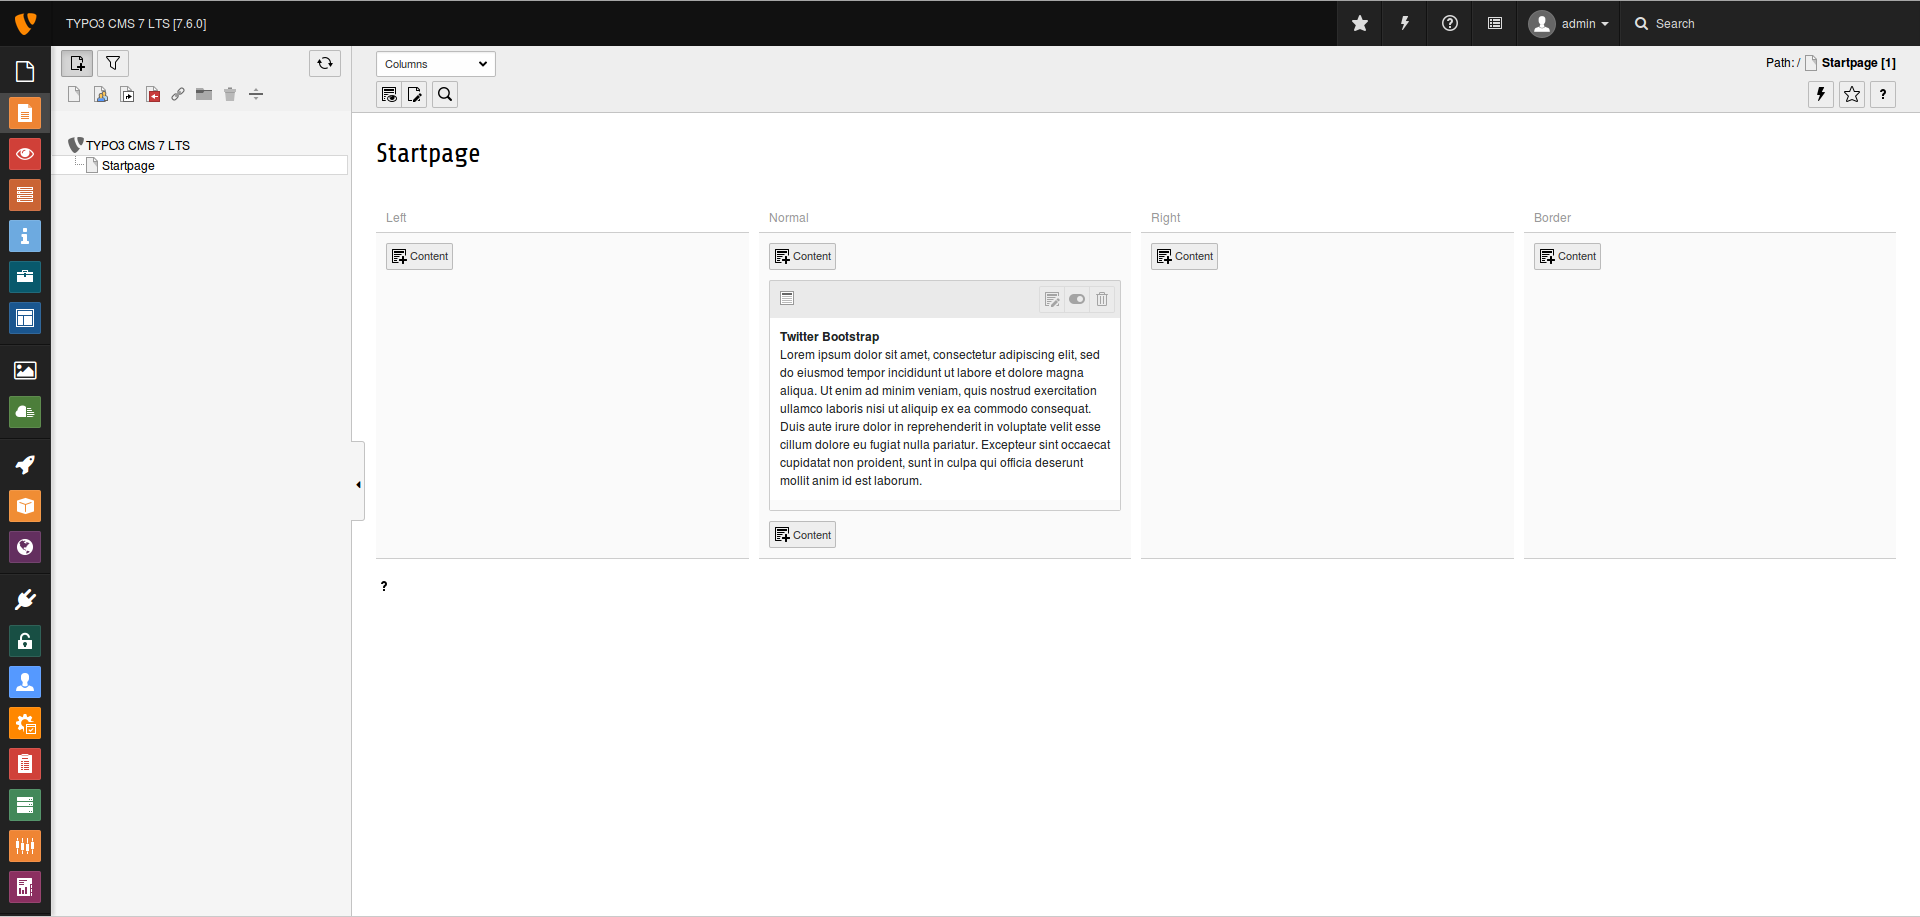
\includegraphics[width=0.90\linewidth]{BackendUserInterface/be-totalscreenshot3.png}
	\end{figure}

\end{frame}

% ------------------------------------------------------------------------------
% LTXE-SLIDE-START
% LTXE-SLIDE-UID:		37ef7143-aeecc039-9d0c10f5-d990bcd8
% LTXE-SLIDE-ORIGIN:	de58d070-98483f3d-0949f2d1-856a9e7e English
% LTXE-SLIDE-TITLE:		Backend User Login
% ------------------------------------------------------------------------------

\begin{frame}[fragile]
	\frametitle{Backend / Внутренний интерфейс}
	\framesubtitle{Авторизация пользователей}

	\begin{figure}
		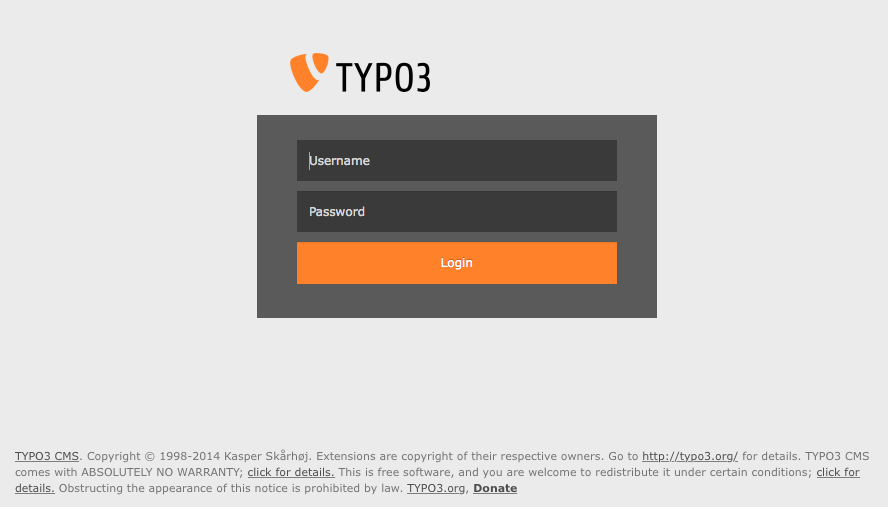
\includegraphics[width=0.80\linewidth]{BackendUserInterface/be-login.png}
	\end{figure}

\end{frame}

% ------------------------------------------------------------------------------
% LTXE-SLIDE-START
% LTXE-SLIDE-UID:		2afbe3a7-2f97d387-01ec7c2a-cacc05e8
% LTXE-SLIDE-ORIGIN:	9baa13c8-78b2f416-28da8e3d-b234e7dc English
% LTXE-SLIDE-TITLE:		Refactor & recolor Modul Menu (Bootstrap)
% LTXE-SLIDE-REFERENCE:	https://forge.typo3.org/issues/62353
% ------------------------------------------------------------------------------

\begin{frame}[fragile]
	\frametitle{Backend / Внутренний интерфейс}
	\framesubtitle{Основная панель (меню модулей)}

	\begin{figure}
		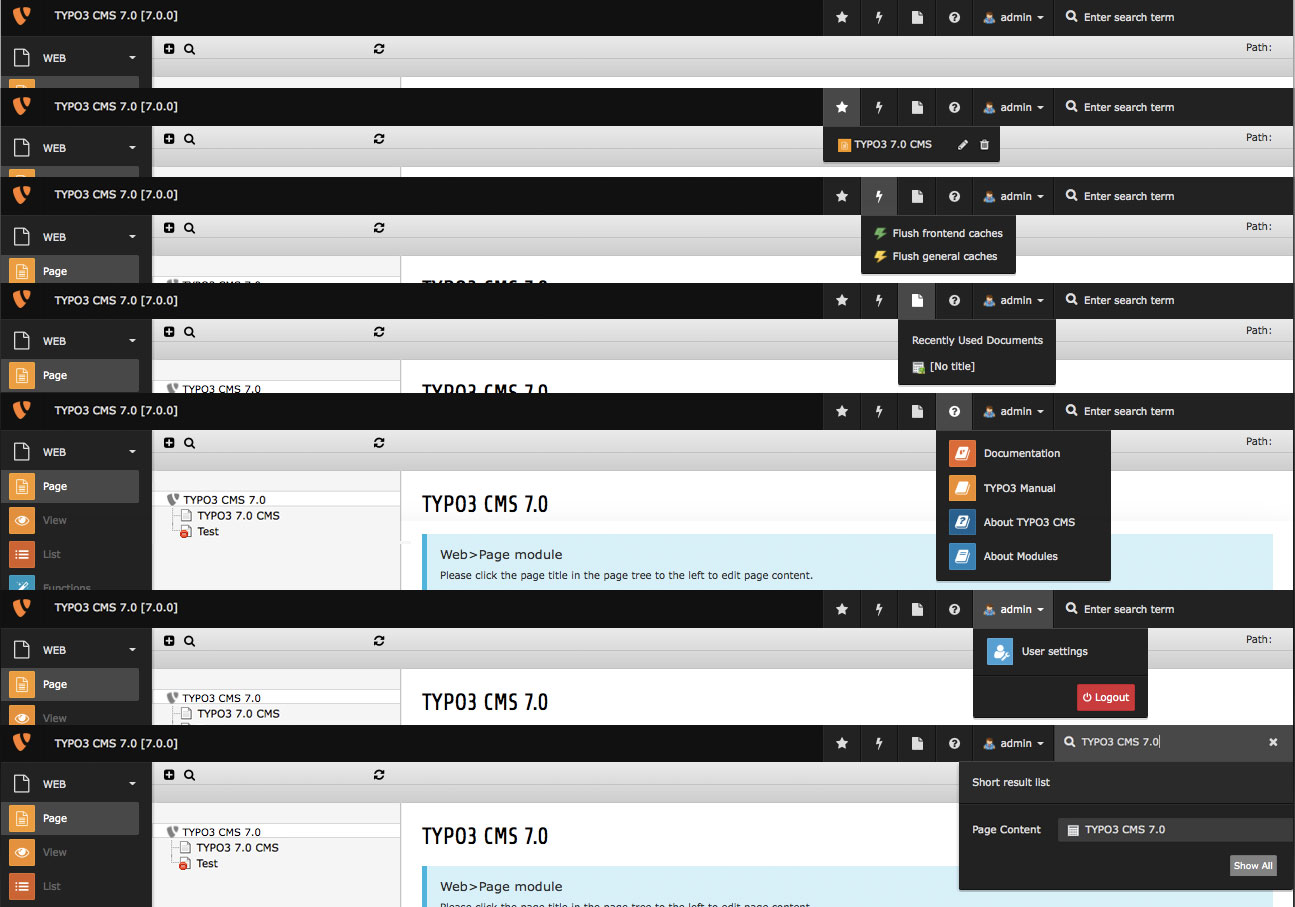
\includegraphics[width=0.70\linewidth]{BackendUserInterface/be-topbar.jpg}
	\end{figure}

\end{frame}

% ------------------------------------------------------------------------------
% LTXE-SLIDE-START
% LTXE-SLIDE-UID:		fc2ddda9-d98ecaf5-78ff10ea-6959c5b3
% LTXE-SLIDE-ORIGIN:	4369ae5e-948d1afa-8212cd72-c91c660b English
% LTXE-SLIDE-TITLE:		New List Module Styling
% LTXE-SLIDE-REFERENCE:	https://forge.typo3.org/issues/62963
% ------------------------------------------------------------------------------

\begin{frame}[fragile]
	\frametitle{Backend / Внутренний интерфейс}
	\framesubtitle{Модуль список и буфер обмена}

	\begin{figure}
		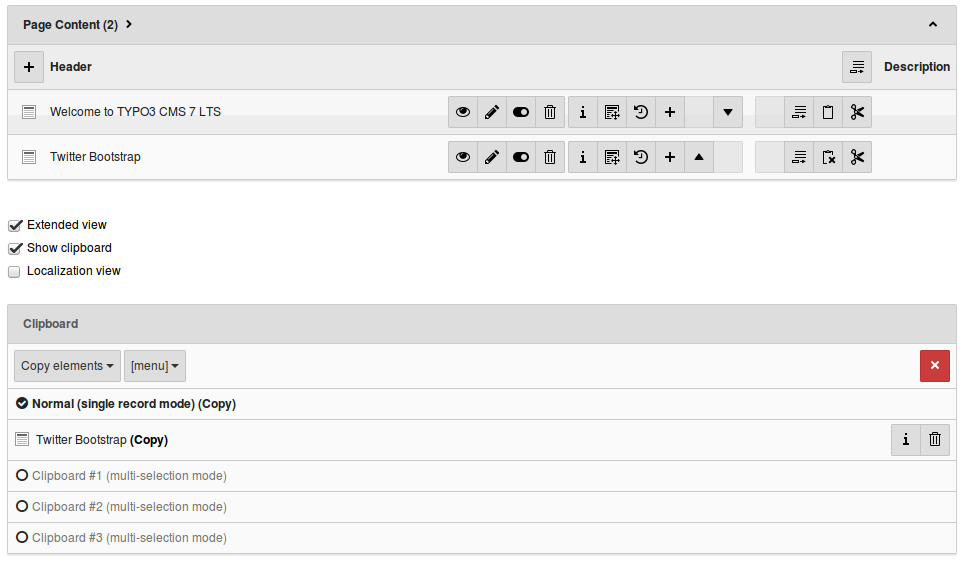
\includegraphics[width=0.80\linewidth]{BackendUserInterface/be-list.png}
	\end{figure}

\end{frame}

% ------------------------------------------------------------------------------
% LTXE-SLIDE-START
% LTXE-SLIDE-UID:		4188f33f-049f31a3-fce5342f-f01f2cd7
% LTXE-SLIDE-ORIGIN:	252361f7-e5c42ec2-a90ecd64-4331f02b English
% LTXE-SLIDE-TITLE:		Table Style
% LTXE-SLIDE-REFERENCE:	https://forge.typo3.org/issues/62159
% ------------------------------------------------------------------------------

\begin{frame}[fragile]
	\frametitle{Backend / Внутренний интерфейс}
	\framesubtitle{Стиль таблиц}

	\begin{figure}
		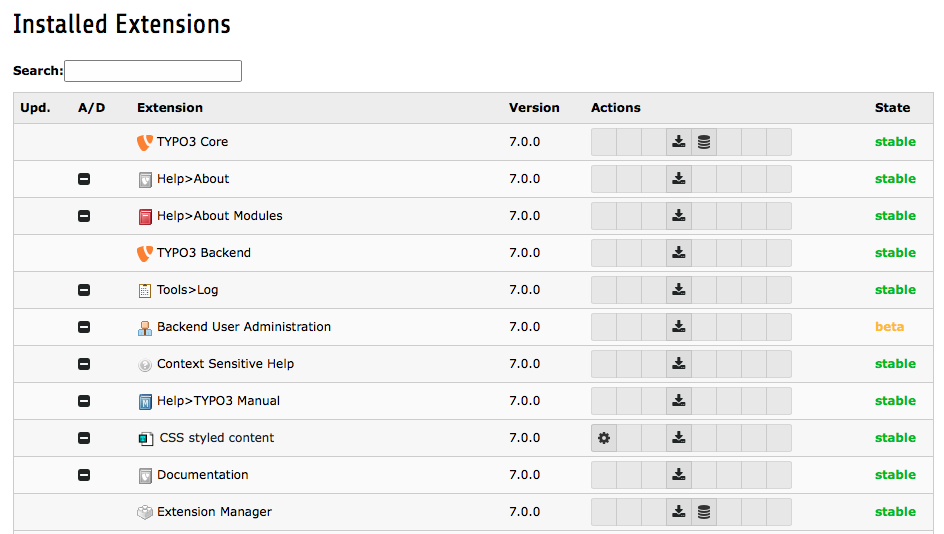
\includegraphics[width=0.99\linewidth]{BackendUserInterface/be-table.png}
	\end{figure}

\end{frame}

% ------------------------------------------------------------------------------
% LTXE-SLIDE-START
% LTXE-SLIDE-UID:		368dfaaf-61a22de3-09109cfc-587269e1
% LTXE-SLIDE-ORIGIN:	785f717d-a7c4d1dd-f186ca6a-060c1dc4 English
% LTXE-SLIDE-TITLE:		Page And List Search
% LTXE-SLIDE-REFERENCE:	https://forge.typo3.org/issues/59763
% ------------------------------------------------------------------------------

\begin{frame}[fragile]
	\frametitle{Backend / Внутренний интерфейс}
	\framesubtitle{Поиск по списку и просмотр страницы}

	\begin{itemize}
		\item Щёлкните по увеличительному стеклу для вывода блока поиска в режимах "список" и "страница"\newline
			(до того функция поиска была в конце страницы)
	\end{itemize}

	\begin{figure}
		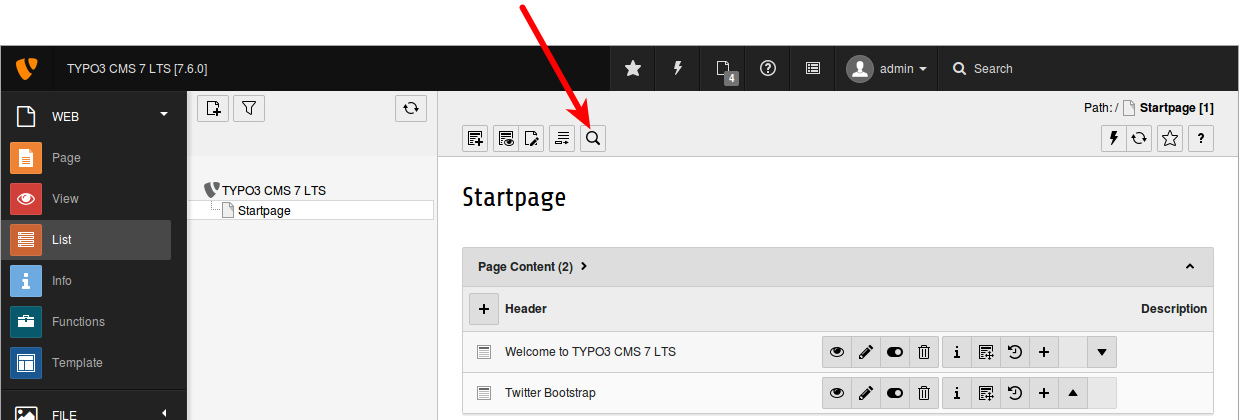
\includegraphics[width=0.95\linewidth]{BackendUserInterface/be-search.jpg}
	\end{figure}

\end{frame}

% ------------------------------------------------------------------------------
% LTXE-SLIDE-START
% LTXE-SLIDE-UID:		13032495-18628a81-fe96833e-cda79742
% LTXE-SLIDE-ORIGIN:	df97fbbf-9ea6c6a9-d9b4c5d4-f8fe1601 English
% LTXE-SLIDE-TITLE:		Migrate Counter of Open Documents to Bootstrap "Badge"
% LTXE-SLIDE-REFERENCE:	https://forge.typo3.org/issues/61675
% ------------------------------------------------------------------------------

\begin{frame}[fragile]
	\frametitle{Backend / Внутренний интерфейс}
	\framesubtitle{Значок с количеством открытых документов}

	\begin{itemize}
		\item Количество открытых документов выводится в виде Bootstrap "badge"\newline
			(требуется системное расширение "Open Documents")
	\end{itemize}
	\begin{figure}
		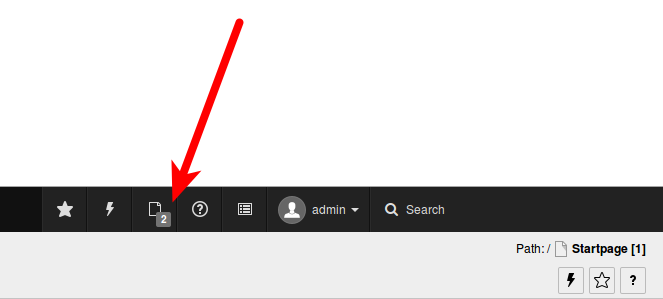
\includegraphics[width=0.75\linewidth]{BackendUserInterface/be-badge.png}
	\end{figure}

\end{frame}

% ------------------------------------------------------------------------------
% LTXE-SLIDE-START
% LTXE-SLIDE-UID:		baaed5a4-dc24f98c-f2f24077-7cbe4ac6
% LTXE-SLIDE-ORIGIN:	a25faae4-8c12c45e-b337b64a-0cf2f53f English
% LTXE-SLIDE-TITLE:		Rebrush FlashMessage
% LTXE-SLIDE-REFERENCE:	https://forge.typo3.org/issues/62580
% ------------------------------------------------------------------------------

\begin{frame}[fragile]
	\frametitle{Backend / Внутренний интерфейс}
	\framesubtitle{Flash-сообщения}

	\begin{itemize}
		\item Обновлён внешний вид Flash-сообщений
		\item Используется контрастный текст на фоне блока
	\end{itemize}

	\begin{columns}[T]
		\begin{column}{.25\textwidth}
			\smaller\hfill 
				\begingroup\color{typo3red}TYPO3 CMS < 7.0\endgroup
			\normalsize
		\end{column}

		\begin{column}{.5\textwidth}
			\begin{figure}\vspace*{-0.6cm}
				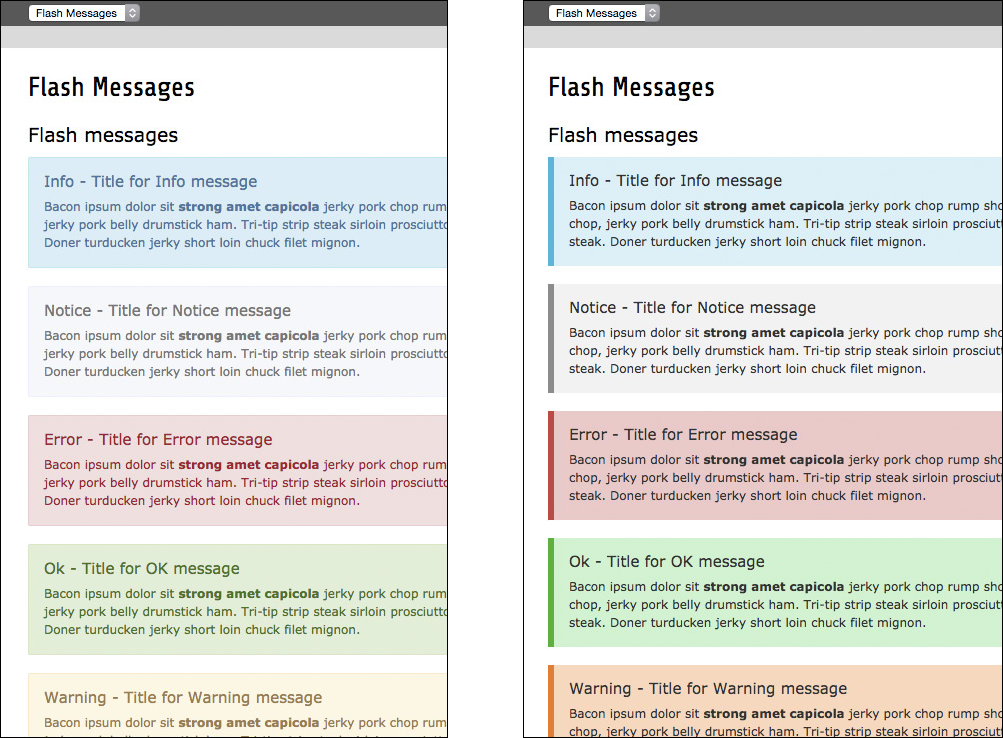
\includegraphics[width=0.99\linewidth]{BackendUserInterface/be-flashmessages.png}
			\end{figure}
		\end{column}

		\begin{column}{.25\textwidth}
			\smaller
				\begingroup\color{typo3red}TYPO3 CMS >= 7.0\endgroup
			\normalsize
		\end{column}

	\end{columns}

\end{frame}

% ------------------------------------------------------------------------------
% LTXE-SLIDE-START
% LTXE-SLIDE-UID:		2aa392c7-6ca76e81-b17c3105-445d1cd0
% LTXE-SLIDE-ORIGIN:	d6a85376-8109aa8c-45a40582-7edb975a English
% LTXE-SLIDE-TITLE:		Video Player in Info Window
% LTXE-SLIDE-REFERENCE:	https://forge.typo3.org/issues/61668
% ------------------------------------------------------------------------------

\begin{frame}[fragile]
	\frametitle{Backend / Внутренний интерфейс}
	\framesubtitle{Видео плеер в окне информации}
	\begin{itemize}
		\item HTML5 аудио и видео файлы можно проигрывать в окне информации\newline
			(где выводятся мета данные)
		\begin{figure}
			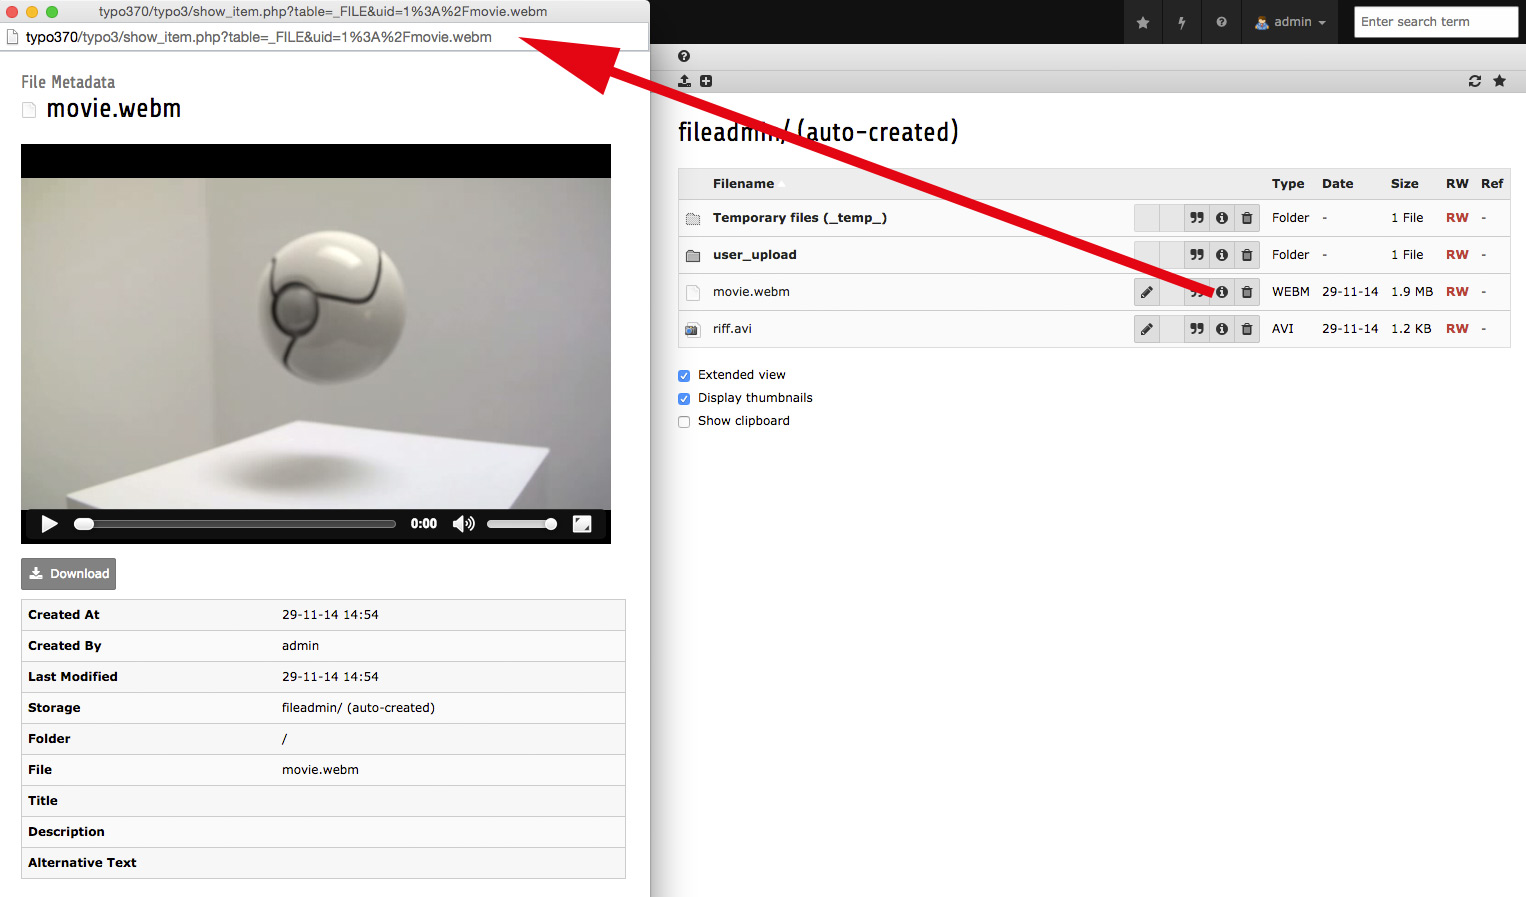
\includegraphics[width=0.70\linewidth]{BackendUserInterface/be-info.jpg}
		\end{figure}

	\end{itemize}

\end{frame}

% ------------------------------------------------------------------------------
